\chapter{System Design}
\label{chap:design}

Our goal is to design a prototypical system that can assist people with dementia during a hand-washing process by assessing their states and provide instructions accordingly. How the instructions are expressed should consider the user's emotional states.

People with certain types of cognitive disabilities have trouble in accomplishing daily tasks. For example, persons with dementia tend to forget where they are in a handwashing task, and without a caregiver's reminder, they might not be able to proceed. However, the need of human assistance in everyday tasks can cause the persons with dementia feeling unconfident and sorry for him/herself. The frustrating caring jobs could also add burden to the families.

An assistive handwashing system is a cognitive intelligent system that can monitor user's behaviours and give proper prompts at certain times. Basically, the system observes the outside world and analyzes the observations over time. At each time step, the system updates its belief states about where the user is at in the handwashing task, and if needed, gives out proper prompts based on these belief states. One limitation of previously-built handwashing systems is that they did not consider users' emotional state changes during the interactions. In other words, the previous systems work functionally, but not emotionally. This defect could limit the effectiveness of the systems when expressing their instructions to human users. The handwashing system we design is able to compute both the user's functional states (i.e. where the user is at during the handwashing process) and emotional states (i.e. the user's identities and emotional states at each time step). The prompts it gives out are produced based on both of the above two states. 

This chapter illustrates how our system is designed as an integration of independent components. Design and implementation difficulties in each component are analyzed in order. Our objective is to design an extensible system that combines affect recognition of behaviours, affective reasoning during interactions, and affective signals generation with AI techniques. This chapter is structured as following. Section~\ref{sec:analysis} analyses the functionality and input/output requirements for each component of the system. It also discusses the difficulties in and proposes possible solutions to designing these components. Section~\ref{sec:design-details} explains how each of the components is actually designed by the selected approach.

\section{Analysis}
\label{sec:analysis}

\begin{figure}[h!]
\centering
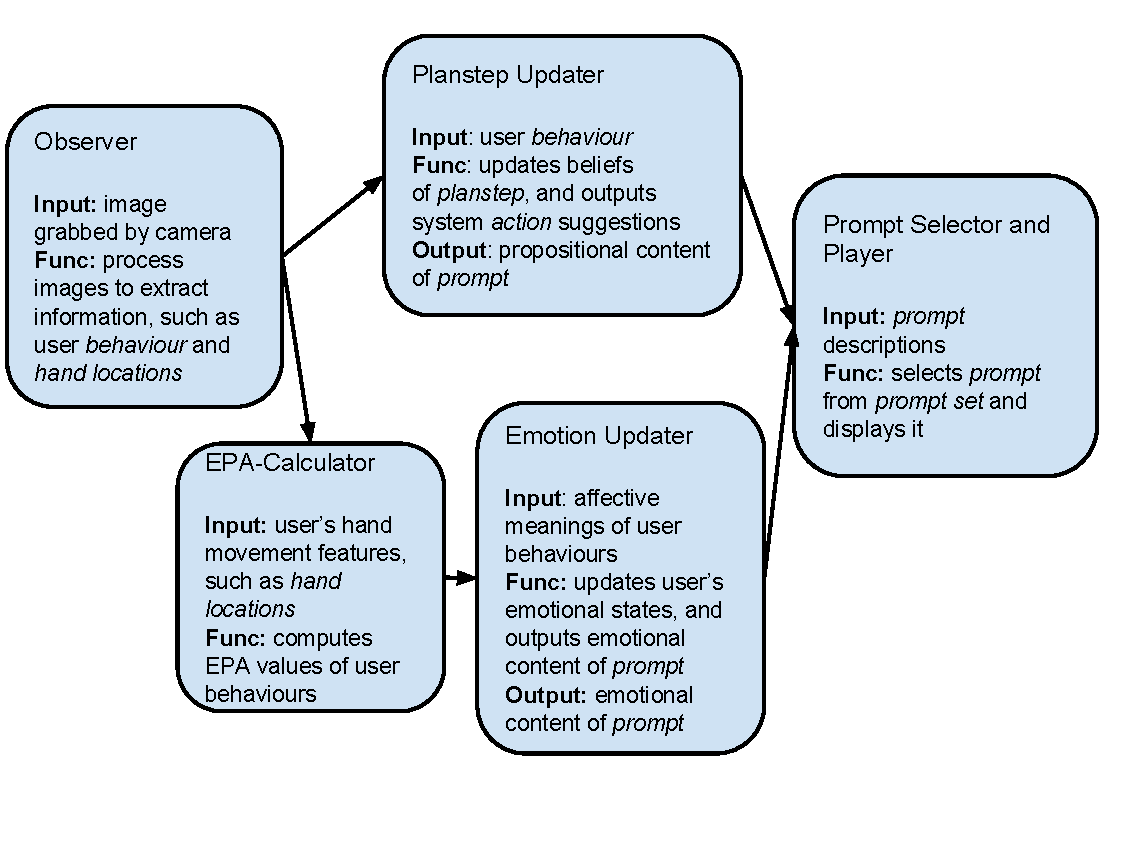
\includegraphics[width=0.9\linewidth]{fig-components.pdf}
\caption{Functionality analysis on the system}
\label{fig:components}
\end{figure}

Figure~\ref{fig:components} describes the essential components of the hand-washing system based on a functionality analysis on the system. It shows also the data flow between components in the hand-washing system. The user's movements are observed and parsed in the \textbf{Observer} to extract information, such as user behaviours (e.g. ``turning on water'') and hand locations (i.e. the coordinates of the user's hands). User behaviours are then fed into the \textbf{Planstep Updater}, where beliefs (probability distributions) of where the user is at in the hand-washing process is updated and contents of instructions guiding the user to proceed is decided. On the other hand, hand movement features (such as hand locations) are fed into the \textbf{EPA-Calculator}, where emotion interpretations of the user's behaviours are computed. The \textbf{Emotion Updater} updates the beliefs of the user's emotional state basing on emotional interpretations of user behaviours, and produces the emotional content of the desired system action. Finally, the \textbf{Prompt Selector and Player} of the system selects/generates and displays proper prompts basing on the descriptions. 

Planstep is used to denote the user's functional state and emotion for his/her emotional state. Prompt, which is an instructional message displayed by the system to the user, is used interchangeably with system action in our descriptions. The rest of this section analyzes the input, output, functionality and design difficulties of these components. For easier description, ``the \textbf{Output Part}'' is used alternatively with ``Prompt Selector and Player'' to refer to the same component.

\subsection{The Planstep Updater}

Planstep denotes the functional state of a user (i.e. how much has he/she accomplished) during the handwashing task. A set of subtasks of handwashing are defined, and each planstep is a combination of the completeness of these subtasks. For each timestep, the system checks if particular behaviours have been performed and updates planstep beliefs if particular subtasks are accomplished. A general definition of subtasks involved in a handwashing process uses three indicators: whether the water is on (on/off), the soap is on user's hand (dirty/soapy/clean), and the user's hands are wet (dry/wet). The corresponding planstep update diagram of this definition is shown in Figure~\ref{fig:planstep}.

\begin{figure}[h!]
\centering

\includegraphics[width=0.8\textwidth]{fig/planstep.png}
\caption{A planstep update diagram. Integers 0 to 7 denote the eight plansteps this subtask partition defines, which are (0) ``off/dirty/dry'', (1) ``on/dirty/dry'', (2) ``off/soapy/dry'', (3) ``on/soapy/dry'', (4) ``on/clean/wet'', (5) ``off/clean/wet'', (6) ``on/clean/dry'', (7) ``off/clean/dry'', respectively. A1 to A5 represent five behaviours completing the subtasks. A1 to A5 are ``turn on water'', ``put on soap'', ``rinse hands'', ``turn off water'', and ``use towel'', respectively.}
\label{fig:planstep}
\end{figure}

Estimating if a subtask has been accomplished in the handwashing process is the most essential part in the planstep update. This can be broken down into two subproblems: (1) to check if an user behaviour has been performed; (2) to decide if a subtask has been accomplished accordingly. Note that the first subproblem is solved in the Observer in our approach.

Usually, sensors are put around the sink area to collect supportive evidence on recognizing user behaviours. One typical approach is vision-based \cite{hoey2006tracking, mihailidis2004use, czarnuch2014}: a camera is mounted above the sink to capture images of the area. For each video frame, by analyzing on the captured images, hands are tracked and their coordinates are obtained. By comparing the positions of the user's hands with the predefined ones of objects (such as soap, towel, sink and water), a system is able to check if the user's hands are within the neighbourhood of a certain object. If a certain area is detected, then the corresponding user behaviour is implied. For example, if the user's hands are detected to be in the neighbourhood of the soap, then he/she is believed to be putting on some soap on his/her hands. 

Note that even if the hand locations are extracted without errors (which in reality is impossible), this location-based approach still can not claim to have 100\% accuracy in detecting user behaviours. This is because having put one's hand in a particular position does not necessarily imply that the person is performing a certain behaviour. For example, the user can simultaneously put his hand on the tap while doing nothing, where a behaviour of ``turning on water'' or ``turning off water'' would be false positively detected by this approach. Adding more sensors (such as pressure sensors for detecting waterflow) might increase the accuracy of user behaviour detection; however, too many sensors is undesirable in our system design. Similarly, due to the subjective nature of the problem, having performed a behaviour does not necessarily imply the completeness of a subtask. For example, even though the behaviour of ``using the towel'' is detected, the dryness of the user's hands is still not predictable without further information. 

Given the partially observable nature of user behaviours and the non-deterministic relationship between user performing a behaviour and user accomplishing a subtask, the Planstep Updater is designed based on the POMDP model and as an extension to the BayesAct engine \cite{hoey2013bayesian} in our approach. To model the observation noise and the uncertainty between user behaviours taken and subtask completeness, a probability distribution is associated with each observation and possible behaviour. The probability distribution associated with observations gives the probability that one user behaviour is detected while another user behaviour is actually being performed. The probability distribution associated with behaviours, on the other hand, gives the probability that a subtask has been completed by the user when a certain behaviour is performed. With these two probability distributions, the Planstep Updater is able to update planstep beliefs based on user behaviour observations. Given the planstep of a user, the functional content of the system prompts is then decided based on a policy. Section~\ref{sec:design-details} and Chapter~\ref{chap:impl} of this thesis describes in more details the design of the Planstep Updater, and the policies used to compute functional content of prompts.

\subsection{The Emotion Updater}

The Emotion Updater in our approach is designed based on the BayesACT model. Three-dimensional vectors that represent evaluation, potency, and activity (EPA) respectively are chosen to describe affective meanings in our work. Basic concepts of both of BayesACT and ACT are introduced in Section~\ref{sec:concepts} of this thesis. As explained there, ACT can serve as a general psychological principle of micro-regulation of interpersonal interactions and BayesACT is able to learn the identities of users from their behaviours.

According to ACT, large deflections between the immediate impressions of the system prompts have on the user and the user's fundamental sentiments of him/herself and the hand-washing system would cause the user's attention to shift away from the premium communication objectives (i.e. to have his/her hands washed). Thus, it is important for the system to act in a way that is aligned with the user's emotional states. For example, if the user thinks of himself as the ``boss'' in their interaction, a more polite suggestion rather than an order should be given to achieve effective communication. Unfortunately, diseases can cause identity shifts \cite{lively2011identity}, and the identity of a person with dementia is not obvious at all \cite{orona1990temporality, rose2004memory}. Therefore, the user's identity should be learned from his/her behaviours. By representing the identity belief of the user as a probability distribution and updating it using observation functions, where the observations are emotional interpretations (i.e. EPA values) of user behaviours, the Emotion Updater designed based on the BayesACT model is able to learn the user's identity. How exactly the Emotion Updater is designed in our system is explained in Section~\ref{sec:design-details}.

\subsection{The EPA-Calculator}

The BayesACT model does not tackle the problems of affect recognition and generation. Thus, for it to be used, an ``input mapper'' measuring the EPA values of user behaviours, as well as an ``output mapper'' mapping the propositional and EPA-vector descriptions of the system's guidance messages into concrete prompts are needed. The ``input mapper'' corresponds to the EPA-Calculator discussed in this subsection, and the ``output mapper'' corresponds to the Output Part of the system, which will be discussed later.

The problem of affect recognition from human behaviours, including affect recognition from bodily movements, facial expressions, sentences spoken, etc, is a large set of machine learning problems. A standard process of solving a machine learning problems consists of feature selection, data collection and labeling, model training and testing. Since affect recognition is still an explorative research area, each of these processes can be a challenge problem itself. Chapter~\ref{chap:bg} of this thesis reviewed some of the previous works in recognizing affect from user behaviours; however, constrained by the specialty of our application scenario --- to assist people with dementia (i.e. special user group) during hand-washing process (i.e. special use case where user's verbal and facial expressions can not be obtained easily and/or clearly), few of the previous approaches fit into our system naturally.

Recognition studies from facial expression analysis, which are relatively mature approaches, are not suitable for our application scenario. There are several reasons for this. Firstly, most facial expression analysis methods are based on data sets consisting of acted expressions; even though for approaches where spontaneous expressions are used, the expressions are performed by normal healthy persons rather than persons with dementia, the user group of our hand-washing system. Since diseases could cause physical changes (e.g. persons with dementia might have fewer facial expressions), the performance of the facial expression analysis methods claimed to have high accuracies elsewhere might not remain the same when applied to our application. Moreover, most existing approaches analyzes clear front-view facial expressions, which is difficult to obtain during the handwashing process. 

Acoustic-based methods recognizing affect by analyzing acoustic features, words spoken, or even sentence structures have been examined by studies as well. However, speech recognition for elderly persons is harder than for younger people, and dementia can cause additional difficulties. Also the ambient noises (e.g. water running) can be a possible problem. Thus it is not feasible to collect user voices clearly during the hand-washing process, not to mention that extracting and analyzing words selected and sentence structures from audio recordings is itself a big challenge. 

While one possible approach to deal with the user-group constraints of our application is to select features by cooperating with sociologists, psychologists and physiologists, and to collect and label data, a large amount of time, effort and expertise would be required in this approach. With its focus on building a prototypical system integrating emotional intelligence, this thesis project did not go through these complicated processes. Features that do not require a large amount of complicated sensors are selected in our system. To be more specific, the expansiveness between user's hands and the velocity of the user moving his/her hands are the features chosen in the system for computing affective meanings (potency and activity, to be specific) of user behaviours. This selection is supported by previous studies. For example, in the work of Beck and his colleagues \cite{beck2010interpretation}, the authors derived a relationship between motion parameters and affective state, and showed that velocity and expansiveness correlate with arousal.

In our approach, a camera is mounted above the sink area and the information needed by the EPA-Calculator (i.e. hand locations) is extracted by the Observer through vision-based techniques. More features (and their corresponding sensors) might need to be added to the system if the EPA-Calculator is extended in the future.The calculated EPA representations are then fed into the Emotion Updater where the system's belief states about the user's identities are updated. Based on the belief states, the Emotion Updater then produces the affective meanings required for system prompts according to the principle of minimizing deflection. ``The affective meanings required for system prompts'', i.e. how the system prompts should be expressed, is represented as EPA vectors in the system. For easier description, we refer to this as the ``emotional description of system actions'', or the ``emotional actions of the system''. More discussions of the Emotion Updater component can be found in the Section~\ref{sec:design-details}.

\subsection{The Observer}

The Observer perceives the world by sensors and extracts information required by the updaters. What sensors should be mounted and what information should be extracted depends on the input requirements of the Planstep Updater and the EPA-Calculator. As mentioned in the above analysis of the Planstep Updater and the EPA-Calculator, in our system, the Observer grabs images using a camera mounted above the sink area, recognizes and tracks the user's hands using vision-based techniques, and extracts the user's behaviours using a location-based method.

To obtain the hands locations and the user's hands movement, a 4D (RGBD) camera is mounted above the sink area to grab images for later analysis. A 4D camera is better than a normal camera in the sense that it is able to get depth information of objects as well. With this additional information provided, image analyzers are able to achieve more accurate results. In fact, it would be difficult for the analyzers to differentiate the vertical distances between the user's hands and certain objects without depth information, in which case the user would be detected as ``using the soap'' whenever his/her hands and the soap are projected at the same place on the x-y plane (regardless of what the z values are). 

\begin{figure}[h!]
\centering
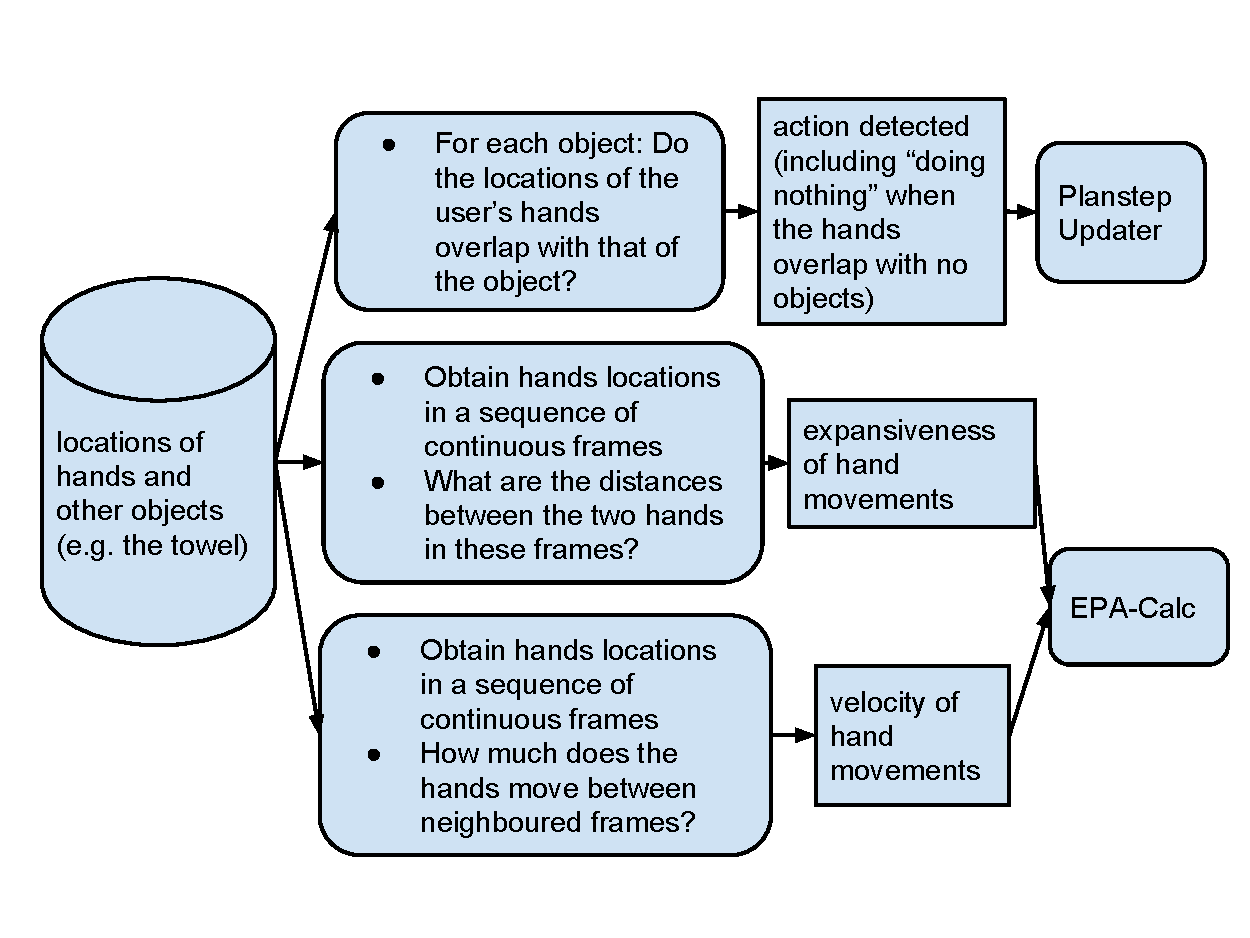
\includegraphics[width=0.9\linewidth]{fig-location-use.pdf}
\caption{How the location info of hands and other objects are used in the system}
\label{fig:location-use}
\end{figure}

Figure~\ref{fig:location-use} shows how the location-based method used in our design maps the location information of the user's hands to user behaviours and how it uses this information to compute expansiveness and velocity of the user's hand movements. As shown in the figure, the location-based method detects user behaviours by comparing the locations of the user's hands with those of the objects we are interested in \cite{boger2005decision, czarnuch2014}. With pre-defined coordinates of certain objects (e.g. the soap, the towel, etc), an user behaviour (e.g. ``using the towel'') is said to be detected if the corresponding object (e.g. the towel) is close to the user's hands. If multiple objects are close to the user's hands, then the closest one is selected. Apparently, the range at which the hands are considered ``close enough'' to an object should be designed carefully. At least the ranges should be different for different objects. 

To be more sophisticated, as opposed to being a constant value, the range associated with an object in the location-based method could even be implemented as a probability distribution describing the probability of the user's hands touching the object given the distance between the coordinates of hands and the object. In such a case, comparisons between distances would become comparisons between probabilities, and the object that is closest to the user's hands would become the one that has the highest probability of being touched by the user. In the work of Hoey and Poupart \cite{hoey2005solving}, the authors described the probability distribution of user behaviours given hands locations directly as a POMDP observation function. In their approach, given observations of continuous x-y-z positions of the user's hands, the probability distribution of user behaviours was computed by the observation function, which was some Gaussian distribution.

The location-based approach of detecting user behaviours has its limitations, in the sense that observing the user's hands at a position does not necessarily imply that the user is performing a certain behaviour. Including context information, such as which planstep the person is currently at, or utilizing additional sensors, such as the ones to detect water flow changes, might improve the accuracy of behaviour detection for location-based approaches, while apparently requiring too many sensors is undesirable for a system assisting people with everyday tasks. Luckily though, since the Planstep and Emotion Updater is designed and implemented as a POMDP in our system, all this uncertainty of observations is gracefully handled.

Essentially, the Observer needs to recognize the user's hands from grabbed images and obtain the coordinates of the hands. The Background chapter of this thesis reviewed several previous works in tracking human hands, among which Czarnuch and Mihailidis's approach utilized the depth information of images \cite{czarnuch2014}. Their tracker is able to recognize and track the user's hands accurately and is a suitable base for the Observer component of our hand-washing system. Chapter~\ref{chap:impl} of this thesis gives more detailed explanation on the accuracy of the tracker recognizing user's hands.

The user's behaviours obtained by the Observer are then fed into the Planstep Updater and the hand locations into an EPA-Calculator, where the expansiveness between the user's hands and the velocity of the using moving his/her hands, and thus the affective meanings behind the user's behaviours are computed. Currently, only the hand locations of the user is required to be obtained by the Observer. If the updaters and/or the EPA-Calculator are extended and more information is needed from the Observer in the future, more sensors and analyzers will be added to the Observer if necessary.

\subsection{The Output Part}

A prompt is an instructional message the handwashing system gives out suggesting what the user should do next. As discussed before, in order to convey the intent of the instructions effectively to its user, the system should carefully decide how it should express the instructions. That being said, a prompt is defined with two components: the proposition and the emotion. The propositional part represents ``what behaviour the user should perform next'', while the emotional part indicates ``how the instructional message should be expressed''. Two prompts are considered identical only when they contain the same propositional content and are expressed with the same emotion. For example, the audio messages ``please turn on the water'' and ``please put on some soap'' are different prompts, since they contain different propositional contents. The audio messages ``put on some soap now you slowpoke!'' and ``could you please put on some soap?'' are different prompts as well, since they have different emotional interpretations.

While the main functionalities of the updaters are to update the belief states of the user's planstep and emotional state, they also compute the propositional (i.e. what instructions should be given) and emotional (i.e. how the instructions should be expressed) descriptions of prompts. The descriptions are then fed into the output part, where final prompts are either selected from predefined prompt sets or generated dynamically. This falls into the category of affect generation. The output part also displays the final prompts if needed. Note that prompts might not be needed at every timestep. In fact, if the user is performing smoothly by himself/herself, he/she might even get interrupted and confused by prompts. For easier descriptions, an ``empty prompt'' is defined to describe situations where no prompt is needed.

Dynamic generation of affective messages is a large challenge, as exemplified by the literature on embodied conversational agents (see \cite{cassell2000embodied, niewiadomski2013computational}, and the Background chapter of this thesis). Our approach selects the final prompt to display to the user from a set of pre-generated and evaluated prompts. Four most essential questions involved in this approach are: (1) Deciding the format of the pre-generated prompts: should they be video, audio, or textual prompt? (2) Designing the prompts, e.g. the words used in the prompts. If the prompts are audio or video prompts, the tones how the messages are stated should be carefully designed as well. Character gestures and other details might require considerations as well if video prompts are used. (3) Labeling the generated prompts. While it might be easy to label the propositional content of the prompts, labeling the emotional interpretations of the prompts might require additional effort. (4) Selecting the prompt to display basing on the propositional and emotional descriptions at each timestep. 

The effectiveness of different prompt formats depends on lots of variables, including personal preference and physical states of the users. For example, some users might find that videos with more information encoded are more helpful, while some others might not even look at the screen. The performance of prompt formats depends on the users' physical states as well. Ideally, the system should learn users' responsiveness to different prompt formats and select the most appropriate ones, or allow users to set prompt format preferences themselves. The format of audio-visual is used for the purpose of demonstration in our prototype. The format of audio-visual was used in the previous work on COACH system as well.

Prompt design is very important as it directly affects the usefulness of the prompt. The user would have difficulty understanding the system's intent if an ambiguous prompt is displayed. Aside from stating its intent clearly, the system should also encode emotion in the prompts. For example, different character gestures should be used to infer to different emotional interpretations. The more prompts with different emotional interpretations are generated, the more choices from which the final prompt is selected are provided and the more accurate results are expected. However, the number of pre-generated prompts is limited. Thus, the number of prompts pre-generated and the emotional interpretation differences between the prompts both need to be carefully decided. 

This thesis uses the set of audio-visual prompts generated and evaluated in Malhotra's study \cite{malhotra2014} as a prompt dataset and selects the most proper prompt from it. Malhotra designed 30 emotionally aligned audio-visual prompts that could be used by a cognitive assistive system in a handwashing scenario in her study. An empirical survey was conducted by Malhotra to get the prompts evaluated in terms of EPA values. Readers can refer to the Background chapter for more details of Malhotra's study. Given the set of pre-generated video prompts with both propositional and emotional labels, and the propositional and emotional descriptions of desired prompts computed by the Planstep- and Emotion- Updater, the Output Part is able to select a most proper prompt from the set by choosing the prompt with the same propositional labels and the closest emotional labels from the pre-evaluated set. The difficulty of the selection then lies in the definitions of emotional closeness between prompts. The emotional closeness of two prompts is related to the Euclidean distance between their emotional labels (i.e. the EPA vectors representing their emotional interpretations). Readers can refer to Chapter~\ref{chap:impl} of this thesis for more details of the algorithm used in our approach to choose the final prompt from the prompt dataset.

\subsection{Communication between Components}

Some of the components illustrated in Figure~\ref{fig:components} are implemented from scratch, while others are extended from existing open source packages. Depending on how the existing open source packages are implemented, they utilize different techniques (e.g. developed using different languages) and work differently (e.g. run as an independent thread v.s. serving as an API or component). If an open source package is used in our system implementation, it is used as what it is (of course, with some interface wrappers if necessary), which means that it has not been rewritten in languages different from their original implementations, or been rewritten into APIs. There are several reasons for this. Firstly, the original implementations are usually stable. These widely distributed open source packages have already been tested by the developers who developed them and a large amount of users who used them. Secondly, it is easier to extend or maintain the handwashing system by using the open source packages as what they are. In this way, one can easily update the system by replacing the plug-ins to newer versions (possibly with some changes to the interfaces), whenever bugs are found and fixed in the packages, better performance is achieved by newer implementations of the packages, or more suitable packages are found. Thirdly, it saves time and effort to use the packages as what they are. To sum up, using existing packages as what they are is safe, easy to maintain, extend and switch to other packages if needed, and effort-saving.

\begin{figure}[h!]
\centering
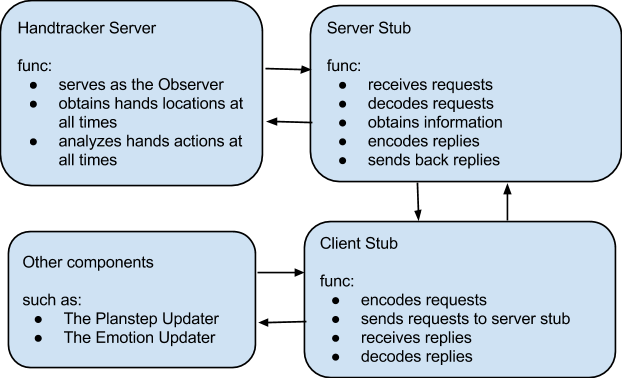
\includegraphics[width=0.8\linewidth]{fig/communication.png}
\caption{Communication between components using server-client model}
\label{fig:communication}
\end{figure}

Now that some of the components illustrated in Figure~\ref{fig:components} are implemented from scratch while others are extended from open source packages, and that the ``plug-in packages'' are used as what they are, coordination between these components becomes a problem. The server-client model can be utilized to communicate between the plug-in packages that run independently and other components. A server stub and a client stub can be developed on both communication parties to encode, send, receive, and decode messages for the two parities. Request and response messages should be defined. While the structures of the two types of messages are not required to be identical, they both should be shared by and accessible to the two stubs. The timings that the client requests and the server replies should be decided as well. This can be explained using the example shown in Figure~\ref{fig:communication}. In the example, a Hand-tracker Server that tracks the user's hands at all times is employed as the Observer component. The Observer detects the user's hand behaviours and feeds them to the Planstep Updater. If the Observer works on a higher frequency than the Planstep Updater, and it sends each user behaviour to the Planstep Updater upon its detection, then more user behaviours than those can be consumed will be sent to the Planstep Updater. Thus, the timings of processing requests and the policies according to which overflowed information is dealt with should be designed carefully. One possible policy is to just drop the exceeded messages; while another solution is to use a buffer to store and pre-process the information. Moreover, when the server and client sides are implemented in different languages, developing a server-client model becomes harder. We will revisit the communication details in the next section.

\section{Design Details}
\label{sec:design-details}

This section explains the design details of the system components in the same order as how they are analyzed in the previous section.

\subsection{The Planstep and Emotion Updater}

The two updaters together decide the functionalities of the Observer and they two together form the functionality center of the hand-washing system. Logically, they both update belief states of the system at each timestep, and compute prompt descriptions based on the beliefs. From an engineering perspective, the two can be combined and developed as a single reasoning engine. In fact, in our approach, the two updaters are implemented based upon the BayesACT model. BayesACT enables machines to generate affectively believable interactions with people by learning about their identity, predicting their behaviours, and taking actions that are simultaneously goal-directed and affect-sensitive. Figure~\ref{fig:updater} shows how this thesis designs the Planstep and Emotion Updater as a single reasoning engine based on the existing BayesAct framework (implemented in \cite{hoey2013bayesian}).

\begin{figure}[h!]
\centering
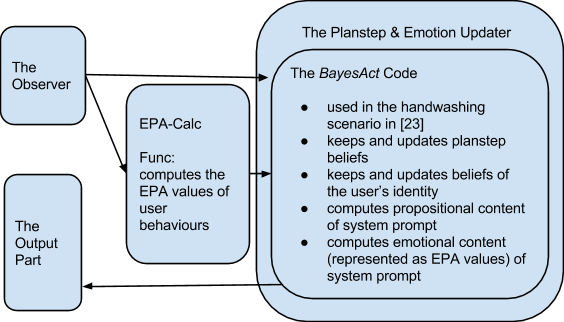
\includegraphics[width=0.8\linewidth]{fig/updater.png}
\caption{Design the Planstep and Emotion Updaters basing on the BayesAct code}
\label{fig:updater}
\end{figure}

Recall that the BayesACT model includes states $S = \{F, T, X\}$, observations $\Omega = \{\Omega_{x}, \Omega_{b}\}$, and agent actions $A = \{A, B_{a}\}$. In our hand-washing system, $X = \{TURN, PS, \\ AW, BEHAV\}$, where $TURN$ describes whether the agent or the client is acting at this time, and $PS$, $AW$, and $BEHAV$ represents the current planstep, awareness and behaviour of the client. The observations $\Omega{x}$ gives evidence to the system about $X$, including evidences indicating which party is currently acting, and what behaviour the client is currently performing if it is currently the client's turn. The system action $A$ denotes the propositional content of a system message. For example, it can be ``to instruct the user to rinse his hands''. $B_{a}$ denote how the message should be expressed. For example, it can be ``state the instructional message with a friendly tone''.

A definition of eight plansteps is used to describe different functional states of the user in a hand-washing process. The corresponding planstep update diagram of this definition is shown in Figure~\ref{fig:planstep}. The current planstep belief $PS$ has eight dimensions, where the $i$-th dimension denotes the probability of the system currently being at planstep $i$. Two probability distributions are used to compute the $PS$ transitions given an observation of the user's behaviour: the distribution $Pr: \Omega_{x} \to \Delta(X_{behav})$ of the user's behaviours over observations, and the distribution $Pr: X_{behav} \to \Delta(X_{ps})$ of the user's functional state moves from one planstep to another after a certain behaviour is performed. $AW$ is a binary variable. It describes if the user is aware or not. A variable $D$ is used to describe the current emotional deflection in the interaction and to infer how responsive a person is to a prompt. $D$ corresponds to the differences between $F$ and $T$. The dynamics in the system are: \\
--- If the user is aware (i.e. has a high $AW$ value), then if there is no prompt from the agent, the user will advance stochastically to the next planstep with a probability that is dependent on the current observation of user behaviour and the deflection $D$. If the user does not advance, she loses awareness (i.e. has a low $AW$ value). \\
--- If the user is aware (i.e. has a high $AW$ value) and is prompted, and the deflection $D$ is high, then a prompt will likely confuse the user and cause his/her have a low $AW$ value. Again, this happens stochastically. \\
--- If the user is not aware (i.e. has a low $AW$ value), then if there is prompt from the agent, and the deflection $D$ is low, the user will likely follow the prompt, which cases the $AW$ value to rise. Otherwise (i.e. there is no prompt, or the deflection $D$ is high), the user will not do anything (or do something else than the one prompted) with high probability.


\subsection{The EPA-Calculator}

To update beliefs of the user's emotional states, the affective interpretations of user behaviours have to be extracted. The EPA-Calculator in the system computes the affective meanings from behavioural features that can be obtained without complicated sensors or pre-processings. To be more specific, the calculator takes a vision-based approach focusing on hands movement analysis.

Threshold-based approaches are used to map expansiveness and velocity levels to potency and activity values of the EPA vectors representing user's behaviours. The evaluation value of the EPA vector remains as default values in this prototypical approach. The EPA-Calculator is designed and implemented as an independent component from the Emotion Updater, which makes it easy to improve the calculator's performances by adding more features or employing new machine learning models without affecting the design of the Emotion Updater and other components in the system. More details on how the EPA-Calculator is designed and implemented in the system can be found in the Implementation and Experimental Results chapter.

\subsection{The Observer}

As discussed in the Analysis section, the Observer of our system uses an RGBD camera mounted above the sink area to grab images and extract features of the user's hand movements. As an extension to the tracker developed by Czarnuch and Mihailidis in their work \cite{czarnuch2014}, the Observer obtains the user's hand locations from images grabbed with depth information by the camera from an overhead perspective. The performance (i.e. the accuracy) of the Observer recognizing and tracking the user's hands is shown in the Implementation and Experimental Results chapter of this thesis. 

After hand locations are obtained, the Observer detects the user's current behaviour and calculates the expansiveness and activity level of the current behaviour basing on the location-based method shown in Figure~\ref{fig:location-use}. In our approach, the coordinates of a set of objects, which are the soap, the towel, the taps, the sink and the running water, are predefined. A behaviour (e.g. ``putting on some soap'') is said to be detected if the user's hands fall into the range of the corresponding object (e.g. the soap). If the user's hands fall into the ranges of multiple objects, the behaviour whose corresponding object is the closest to the user's hands is said to be detected. If different behaviours are detected for the user's two hands, then the final user behaviour is decided using a heuristic policy. Details of this process can be found in the Implementation and Experimental Results chapter of this thesis. The errors caused by the user behaviour detection module are gracefully handled in the system, since that the Planstep and Emotion Updater is designed and implemented as a POMDP.

Currently, only the hand locations of the user is required to be obtained by the Observer. If the Planstep Updater and the EPA-Calculator are improved and require more information as inputs in the future, more functionalities and corresponding sensors should be added to the Observer.

\subsection{The Output Part}

Recall that a prompt, which is an instructional message suggesting what the user should do next, is defined as consisting of two components: the proposition and the emotion. Two prompts are considered identical only when they contain the same propositional content and are expressed with the same emotion. Given the propositional and emotional descriptions of desired prompts computed by the Planstep- and Emotion- Updater, and a prompt dataset of pre-generated prompts with both propositional and emotional labels, the Output Part is able to select out a most proper prompt from the set by choosing the prompt with the same propositional labels and the closest emotional labels from the pre-evaluated set. Our approach uses the set of audio-visual prompts generated and evaluated in Malhotra's study \cite{malhotra2014} as the prompt dataset. Readers can refer to the Implementation and Experimental Results chapter of this thesis for more details of the algorithm used in our approach to choose the final prompt from the prompt dataset.

To utilize the pre-generated and evaluated prompts as a dataset from which the most proper prompt is selected, a file describing all these prompts (e.g. what the labels of each prompt is) is needed. When the system starts, it reads the file and stores the descriptions of prompts and their labels in memory for later use. This thesis project uses a csv file with headers ``filename'', ``prompt\_number'', ``evaluation'', ``potency'', ``activity'' to save information of the prompts. Among all the columns, ``prompt\_number'' is the integral propositional label of a prompt and ``evaluation'', ``potency'', ``activity'' are three real numbers representing the EPA values of the same prompt. 

After a most proper prompt is chosen, the Output Part displays it out to the user. The sub-component that serves as a multi-media player in the Output Part is designed as a VLC\footnote{An introduction to the VLC SDK can be found via \url{https://wiki.videolan.org/LibVLC/}.} SDK application. VLC SDK is a mature and easy-to-use media framework that can be embedded into systems to provide multimedia capabilities for the applications. Minor implementation details, such as the timings to display prompts (e.g. the minimum time length between displaying two prompts), should be decided carefully.

\subsection{Communication between components}

\begin{figure}[h!]
\centering
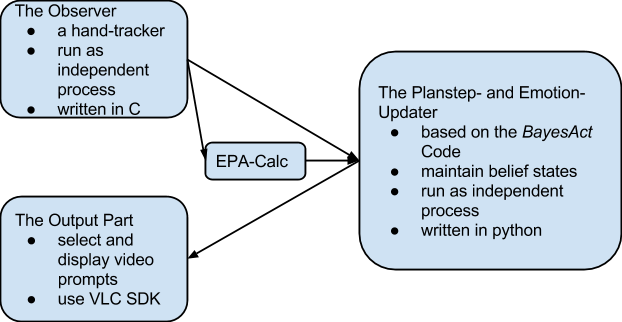
\includegraphics[width=0.8\linewidth]{fig/dataflow.png}
\caption{Data Flow and Logical Relationship between Components}
\label{fig:dataflow}
\end{figure}

Figure~\ref{fig:dataflow} shows an overview of how the system is designed as independent components and how it makes use of existing programs and open source packages. In the system, the Observer component is designed as a hand-tracker based on Czarnuch's tracker \cite{czarnuch2014}, where the original tracker was implemented in C. The Planstep- and Emotion- Updater is designed based on the BayesAct code \cite{hoey2013bayesian}, where the original program was written in python.

Server-client models are utilized to coordinate between the components. To communicate across independent processes and multi-language platforms, server- and client- stubs that receive, decode, encode and send messages are designed. Apparently, the definitions of the messages used in the communications should be shared by and accessible to both the  the server and the client stubs. One way to achieve this is to define message structures on both the client and the server side, and manually ensure that the definitions are identical. This approach is easy to implement; but is vulnerable to bugs and is difficult to maintain. Another approach is to defined the message structures within a single ``header'' file accessible to both of the two sides. The ``header'' file should be referred to in the implementation of both the client and the server side. This approach is safer than the first one, no manual effort is needed to ensure the consistency of messages definitions on the two sides. However, it is infeasible to share same ``header'' files between two components implemented with different languages. A more sophisticated approach is to use Google's protocol buffer mechanism\footnote{Introduction to the mechanism can be accessed via \url{https://developers.google.com/protocol-buffers/}.}, which allows one to define message structures at one place, and to use them at another place. By compiling and automatically generating the definitions in another language, this mechanism ensures the consistency between message definitions shared by both of the communicating sides. The mechanism is also convenient to utilize. It is able to define data attributes in a structure as ``repeated'', ``optional'' and ``required'' fields, which is beneficial to define complicated data types. Useful accessible functions to data fields are provided by the mechanism. Furthermore, since the consistency between message definitions are automatically ensured, message structures defined using this mechanism are extensible.

The timings of the client requests and the server replies should be carefully decided. The components shown in Figure~\ref{fig:dataflow} work with different frequency: the Observer recognizes user's hands, obtains and analyzes hand locations for each frame grabbed by the sensor at a rate about 24 frames/second , while the Updater (extended from the BayesAct code) works as a turn-taking model between the agent (i.e. the system) and the client (i.e. the human user). One solution to solve this problem is to use a buffer between the Observer and the Updater. Information (such as hand locations) obtained from the Observer is saved and analyzed in the buffer. EPA values of user behaviours computed by the EPA-Calculator are as well stored and temporally smoothed in the buffer. How the Buffer temporally smoothes the EPA values of user behaviours are explained in more details in the Implementation section in the next chapter. Messages are sent to the Updater for state updates only when certain conditions are met. Figure~\ref{fig:system} illustrates how the components coordinate with each other with the help of server-client models and such a buffer.

The following three aspects should be carefully designed for the buffer: (1) the conditions which would trigger the buffer to transfer between states; (2) the buffer's size, i.e. the information processed for how many frames can be handled by the buffer; (3) the policy describing how overflowed messages are dealt with. The state machine shown in Figure~\ref{fig:state-trans} illustrates how the buffer is designed in this thesis. As shown in the figure, there are three states of the buffer. State A represents the state where the user performs a same user behaviour within neighbouring frames. Two conditions can trigger the buffer's state to transfer from State A to another state: (1) If an user behaviour different from the current stable behaviour is detected, then the state of the buffer would transfer to State B. If the new behaviour is found to last for less than a \textit{timeup} period, the state of the buffer would change back to State A, with the stable behaviour unchanged. (2) If the buffer has been in State A for a \textit{timeout} period, then the buffer would change to State C, where the state of the buffer would change back to State A immediately after messages encoding the current stable user behaviour are sent to the updaters. State B of the buffer checks if a newly detected user behaviour is a stable one. Similarly, there are two conditions that can trigger the buffer's state to transfer from State B to another state: (1) If the new user behaviour different from the current stable behaviour is found to last for at least a \textit{timeup} period, then the new user behaviour is considered stable. In that case, the state of the buffer would change to State C, where the buffer's state would change to State A immediately after messages encoding this new stable behaviour are sent to the updaters. (2) Otherwise, the buffer's state would change back to State A with the current stable user behaviour non-changed.

\begin{figure}[h!]
\centering
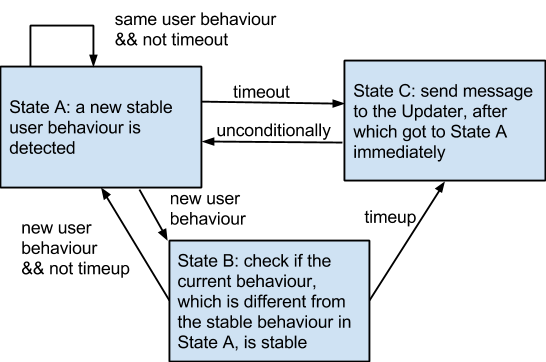
\includegraphics[width=0.7\linewidth]{fig/state-trans.png}
\caption{State transitions of the buffer between the Observer and the Updater}
\label{fig:state-trans}
\end{figure}

\subsection{Summary}

\begin{figure}[h!]
\centering
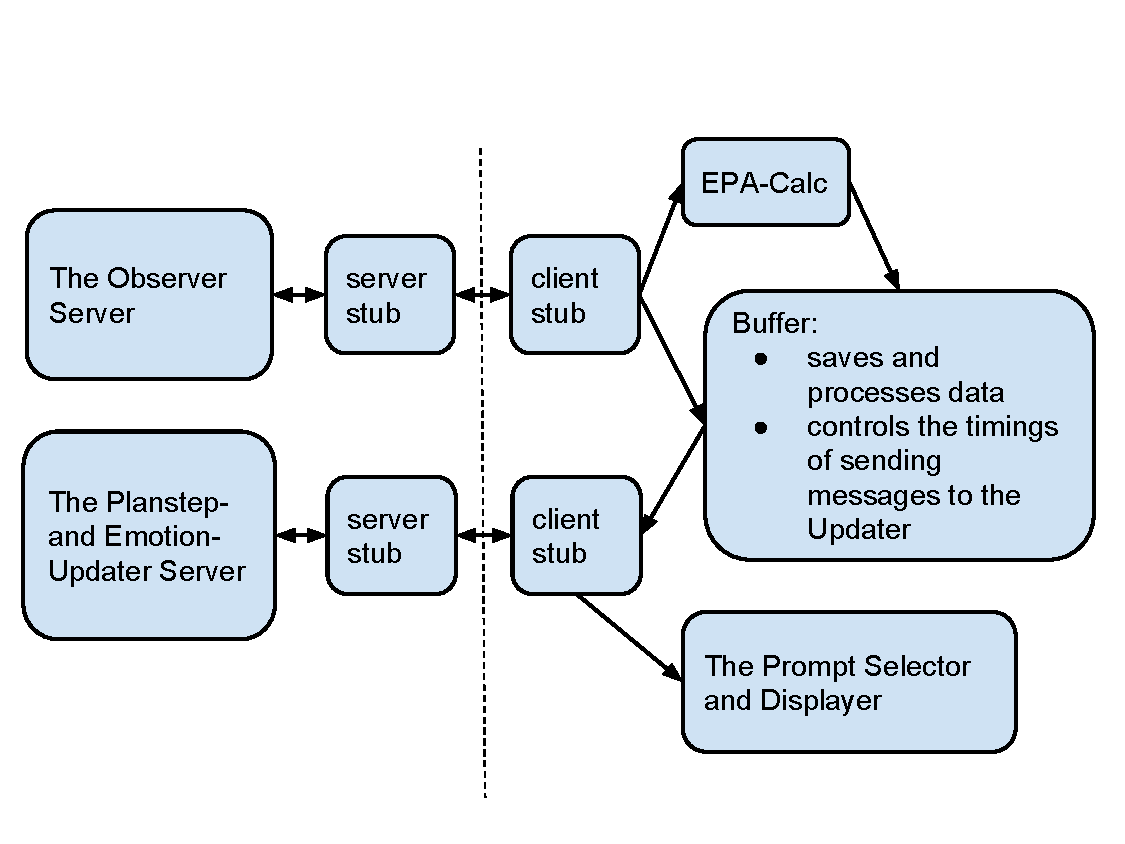
\includegraphics[width=0.9\linewidth]{fig-system.pdf}
\caption{System Design with Server-Client Models}
\label{fig:system}
\end{figure}

To sum up, the system is designed as shown in Figure~\ref{fig:system}. The Observer component of the system is designed based on Czarnuch's tracker \cite{czarnuch2014}, and is used a hand-tracker server. The Planstep- and Emotion- Updater is designed based on the BayesAct code \cite{hoey2013bayesian}, and is used as an Updater server. The rest of the components are designed as client components which communicate with the servers through stubs. Among all the client components, an EPA-Calculator and a Buffer sit between the two servers. The EPA-Calculator consumes user's hand locations and computes the EPA values of user behaviours. The Buffer stores and re-processes user behaviours and their EPA values, and controls the timings at which messages are sent to the Updater server for state changes. How the Buffer temporally smoothes the EPA values of user behaviours are explained in more details in the Implementation section in the next chapter.

Being designed as an integration of independent components, the system is easy to maintain and extend. For example, the Observer Component can be extended to obtain more features useful in computing EPA values for user behaviours without many changes to other components. This system design is portable as well. Since this design enables component communications across processes and multi-languages, one can easily use the same system design (possibly with some minor changes) in other application scenarios.
